%\chapter{spacereq}

%%%%%%%%%%%%%%%%%%%%%%%%%%%%%%%%%%%%%%%%%%%%%%
\section{Installation space and clean room}

Figure \fixme{1} shows the ProtoDUNE SP cryostat in EHN1.  The cryostat will be constructed in a pit inside the building and will be surrounded on three sides by the pit walls.  On the open side of the cryostat we will construct an ISO 8 clean room from which to construct, test and install the TPC.  In addition to air purity, the lighting inside the clean room and any temporary lighting inside the cryostat will be filtered to limit the exposure of the PDs to UV light.  This filtering limits UV less than 450 nm from the ambient light.  

This is also the face of the cryostat that will have the temporary construction opening (TCO) that will allow us to insert and install the large TPC components.  Outside of the clean room is a material pass through or material SAS that will have a removable roof in which to lower the TPC elements into the clean environment from the gallery floor.

\begin{cdrfigure}[short caption for table of figures]{label}{1 long caption that appears below picture}
%  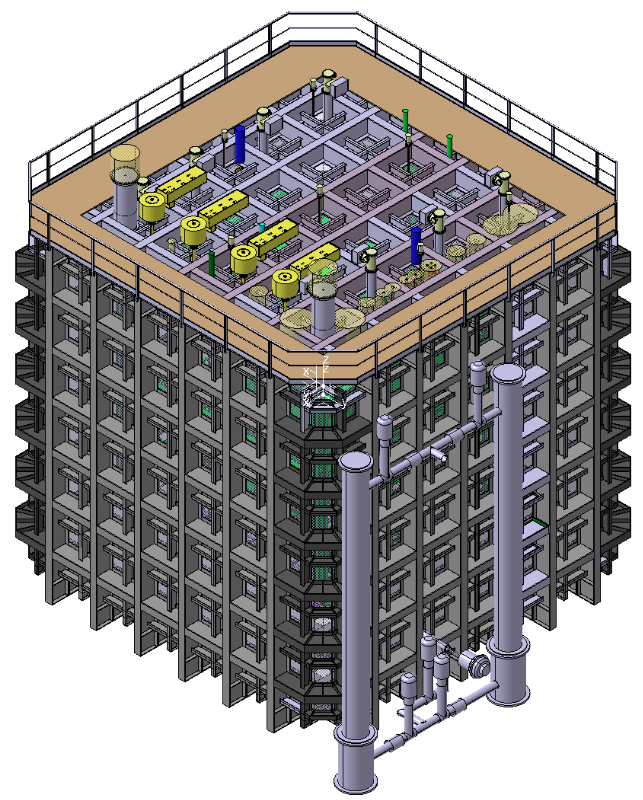
\includegraphics[width=0.8\textwidth]{protoDUNE_cryostat.png}
\end{cdrfigure}

A naming convention has been established to label the four sides of the cryostat for logistical purposes.  The plan view in figure \fixme{2} shows this naming convention.  The upper side is Jura, the lower is Saleve, the left is beam and right is downstream.

\begin{cdrfigure}[short caption for table of figures]{label}{2 long caption that appears below picture}
%  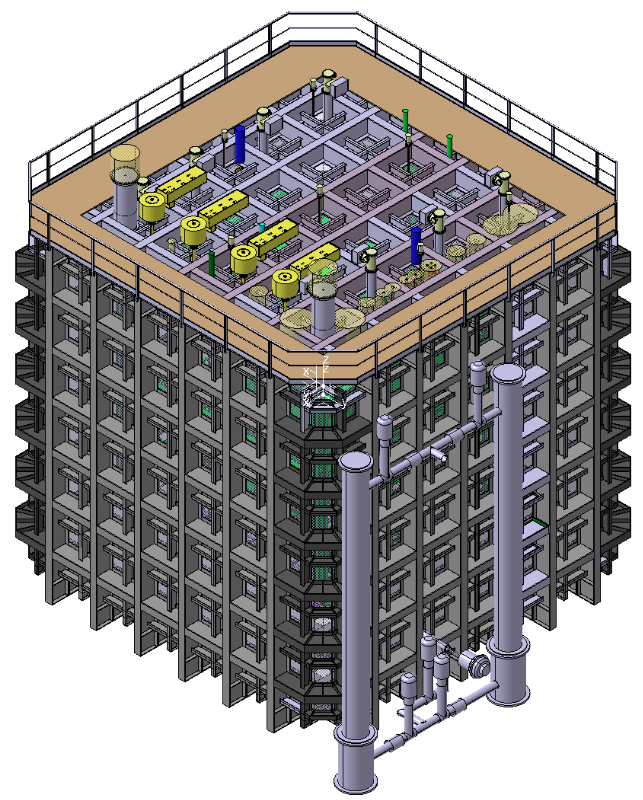
\includegraphics[width=0.8\textwidth]{protoDUNE_cryostat.png}
\end{cdrfigure}

Figure \fixme{3} is an elevation section view of the cryostat.  For reference is shows the position of the TCO and the location of the integrated cold testing stand that will be described in the next section.  The TCO will be used to bring personnel, materials, access equipment and TPC components inside the cryostat. 

\begin{cdrfigure}[short caption for table of figures]{label}{3 long caption that appears below picture}
%  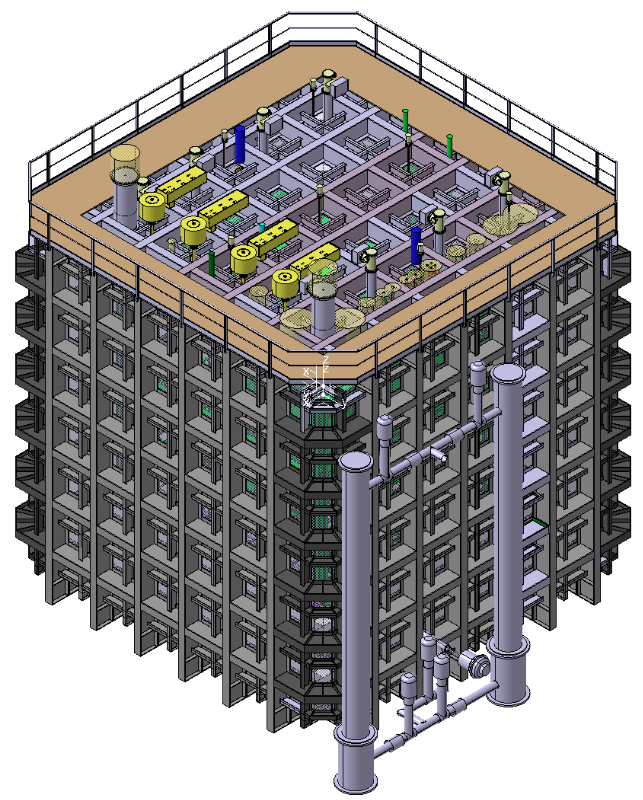
\includegraphics[width=0.8\textwidth]{protoDUNE_cryostat.png}
\end{cdrfigure}


Inside the clean room, there will be a series of rails to facilitate the movement of the TPC components during the test and installation process.  The conceptual layout of these rails are shown in figure \fixme{4}.  These rails will be positioned vertically at the same height of the DSS rails inside the cryostat.  Through the TCO, a temporary rail will be installed that bridges the DSS and the rails in the clean room.  All of the large components of the cryogenic piping and TPC will be supported from these rails on movable trolleys to move them inside the cryostat.  

\begin{cdrfigure}[short caption for table of figures]{label}{4 long caption that appears below picture}
%  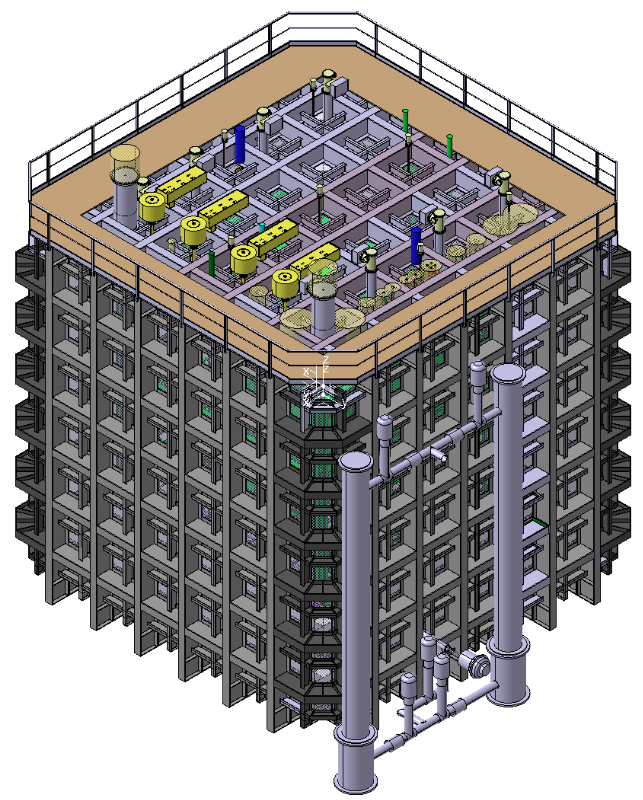
\includegraphics[width=0.8\textwidth]{protoDUNE_cryostat.png}
\end{cdrfigure}


Figure \fixme{4} also shows the approximate dimensions for the material SAS and the footprint of the clean room space.  This space is limited by the pit walls on two sides and the supports for the beam and beam instrumentation on the other.  

Figure \fixme{5} shows the planned locations for all of the activities that will be performed inside the clean room.  
\begin{cdrfigure}[short caption for table of figures]{label}{5 long caption that appears below picture}
%  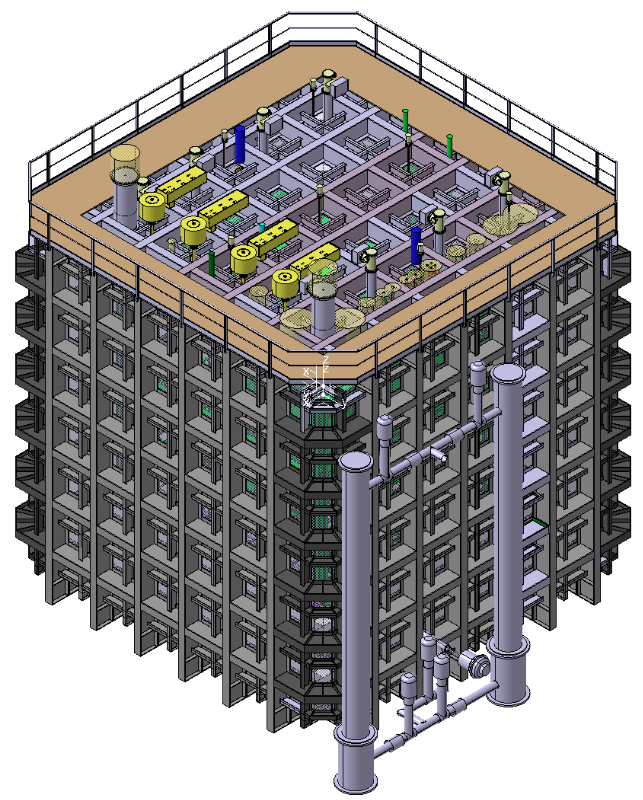
\includegraphics[width=0.8\textwidth]{protoDUNE_cryostat.png}
\end{cdrfigure}
Material will pass through the SAS through a large set of doors.  These doors will be closed while material is lowered into the SAS.  Once the roof of the SAS is closed, these doors will be opened to move the material into the clean room.  This is done to reduce the contamination of the clean room space from the ambient conditions of EHN1.  

The activities planned are as follows:
\begin{itemize}
\item Assembly of the CPA panels into CPA modules.  This requires a large flat surface approximately 1500 mm x 6500 mm to join the three CPA panels into one CPA module.  Once these are assembled, an overhead hoist located near the TCO will be used to translate the CPA module from horizontal to vertical and place it for attachment to the clean room rails.  
\item Attachment of the upper and lower FC assemblies to the CPA modules.  Once two of the CPA modules are attached to the clean room rail, two upper and two lower FC assemblies will be attached.  This will be done with the same overhead hoist located near the TCO.
\item Installing the PDs in the APA frames.  Each PD module will be unpacked, tested and then installed in the APA frame. 
\item Mounting of the CE onto the APAs.  Each of the CE modules with cables will be unpacked, tested and then mounted onto the APA frame.  
\item Integrated testing of APA with PD and CE.  
\end{itemize}

%%%%%%%%%%%%%%%%%%%%%%%%%%%%%%%%%%%%%%%%%%%%%%
%\section{QA/QC and testing space}
\section{Testing}

All of the testing for the TPC components will be done inside the clean room or inside the cryostat.  This will be described for the major sub system components below.
Once the APAs are moved into the clean room, a connectivity test will be performed to look for shorted or broken wires.  It will also be inspected visually for broken wires.  Tension tests will be performed on some fractions of the wires and the results will be compared to the ones taken at the production facility.

For the PDs, each PD will be unpacked and placed inside a full length dark box with a scanning VUV light source. This will be an identical test set up to the one used at the production facility.  Each test will take approximately 2 hours, which is the planned time for the installation and cabling of a PD into the APA.  

The CE modules will be delivered as an assembly.  The CE enclosure will have the electronics boards mounted inside and the internal cable from the harness connected and tested.  Each module will undergo an acceptance test when they are unpacked inside the clean room.  Once tested, they will be installed on the top of the APA frame from either a scaffold or a scissor lift located in the clean room.  A connectivity test will be performed on each module to ensure the electrical connections.  

After the APA has been fully integrated with the PD and CE, it will be moved via the rails in the cleanroom to the integrated cold testing stand.  This test stand, shown in Figure \fixme{6}, is a large insulated box that is light tight for PD testing and a Faraday shield for CE testing.  The test stand is shown with an APA inside and the end cover removed.  
%
\begin{cdrfigure}[short caption for table of figures]{label}{6 long caption that appears below picture}
%  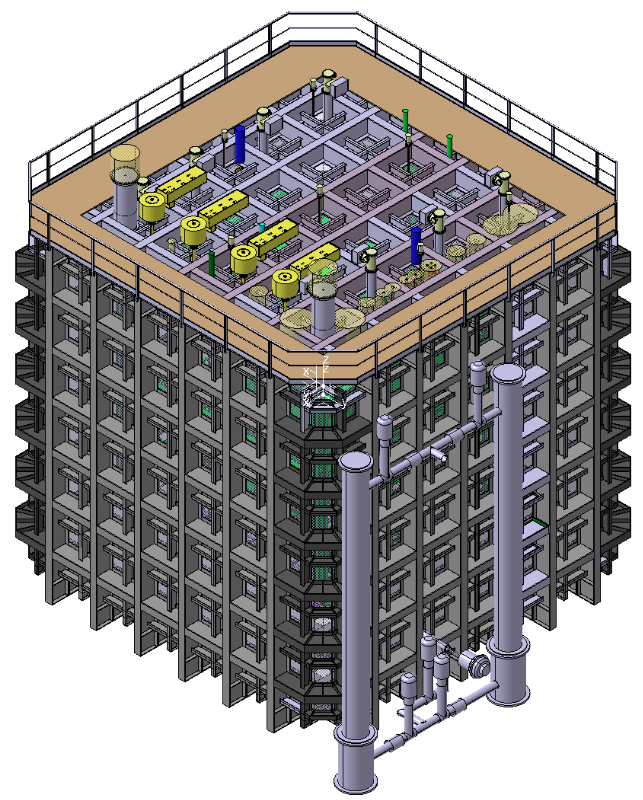
\includegraphics[width=0.8\textwidth]{protoDUNE_cryostat.png}
\end{cdrfigure}
%
At the top of the box, there will be a crossing tube, similar to those in the cryostat, with a conflat fitting that will accept the warm – cold interface flange for the PD and CE cable connections.  The PD and CE cables will be routed and connected to their flanges, the APA will be moved inside and the end cover, that completes the Faraday cage, installed so that the integrated electronics testing can begin.  A series of warm tests will be performed.  This is described in \fixme{XXsectionXX}.  After the warm tests are complete, the inner volume of the enclosure will be purged with dry gas to reduce the moisture inside.  After this gas purge, the inner volume will be slowly cooled down using nitrogen gas to a temperature of approximately 100 K.  The rate of cooldown is to be less than 10 K/hr which is the same for the cryostat.  The cooldown system is being designed to maintain the inner volume near 100 K for approximately 48 hours.  The cold testing of the can be performed during the cooldown period, during these 48 hr and during the warmup.  After the testing is complete and the box has been purged of nitrogen with room air, it will be opened, the APA removed and he cables disconnected and secured for movement on the rail system.   

Each of the CPA panels will be visually inspected for damage to the resistive coating on the panels.  At the panels are assembled into a CPA module, electrical connections will be made and tested between the panels.  As the modules are mounted on the clean room rails, the modules will be electrically connected between the modules.  This connection will be tested in the clean room and when the CPAs are moved inside the cryostat to their final position.  

The FC assemblies will be visually inspected for damage as they are removed from their shipping containers.  The electrical connections between the divider chains will be tested.  Once attached to the CPA, an electrical connection between the CPA and FC must be made to carry the HV to the FC.  This will be tested in the clean room before moving the assembly into the cryostat. 


%%%%%%%%%%%%%%%%%%%%%%%%%%%%%%%%%%%%%%%%%%%%%%
\section{Control room}

One of the barracks located in the EHN1 gallery on a raised platform will be used as a control room for ProtoDUNE SP.  This is shown in figure 7.   Racks will be installed inside the control room for XXX.  Services from the detector and detector racks will be installed and routed through the services trenches located in EHN1.  The location of these trenches are shown in figure \fixme{7}.  
%
\begin{cdrfigure}[short caption for table of figures]{label}{7 long caption that appears below picture}
%  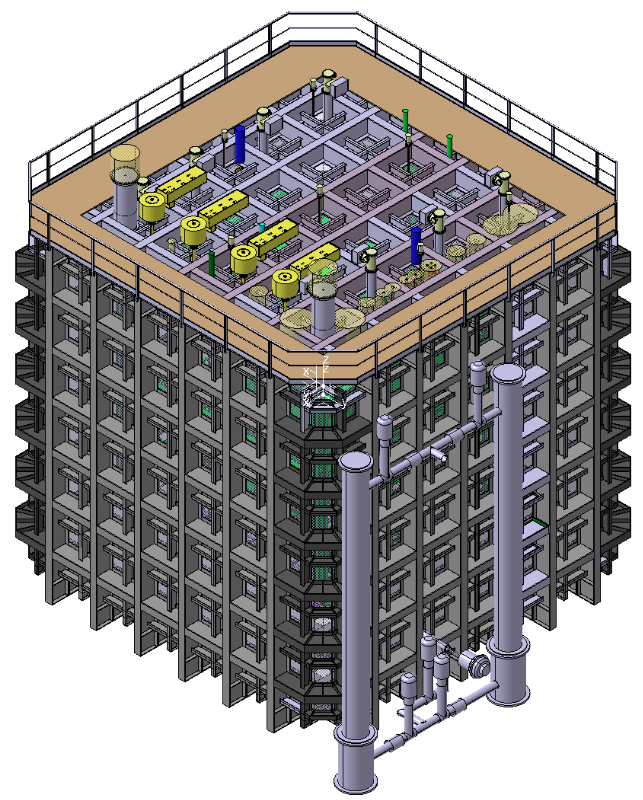
\includegraphics[width=0.8\textwidth]{protoDUNE_cryostat.png}
\end{cdrfigure}
%

%%%%%%%%%%%%%%%%%%%%%%%%%%%%%%%%%%%%%%%%%%%%%%
\section{Infrastructure requirements}

The electronics racks will be located on the gallery floor close to the cryostat as shown in figure \fixme{8}.  Their proximity and location was determined to minimize the cable lengths from the feed throughs on the cryostat.  These racks will be air cooled.  
%
\begin{cdrfigure}[short caption for table of figures]{label}{8 long caption that appears below picture}
%  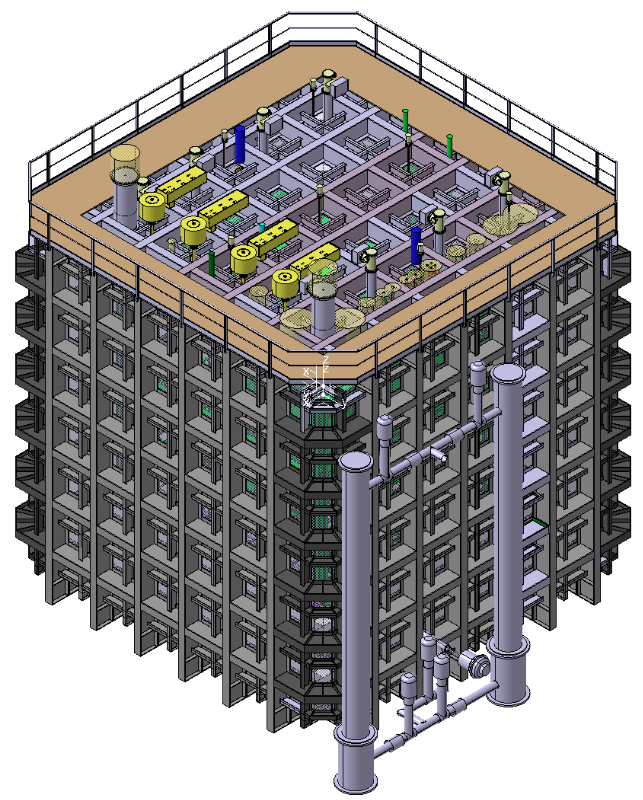
\includegraphics[width=0.8\textwidth]{protoDUNE_cryostat.png}
\end{cdrfigure}
%

%%%%%%%%%%%%%%%%%%%%%%%%
\subsection{System grounding}

To ensure adequate sensitivity of the detectors, special ground systems must be put in place which will “isolate” the detectors from all other building electrical systems and equipment.  The aim is to minimize the influence of inductive and capacitive coupling and ground loops.  Any stray currents seen by the detectors, will increase system noise and adversely affect the S/N ratio.  A single MIP of ~530 electrons collected over 500ns, represents a current of less than 0.2 nanoamperes.  For protoDUNE, the isolated ground will reduce or eliminate ground currents through the detector.

The isolated ground system must also protect both personnel and equipment by providing a low impedance path for equipment short circuit and ground fault currents.  This will be accomplished through use of a saturable inductor which provides the connection between the detector and building grounds.  The inductor saturates with flux under low frequency high current and has minimal impedance to any type of AC power fault current; thus, shunting any fault current to the building ground.  Low current high frequencies signals, such as coupled noise currents, will see the inductor as a high impedance, which will restrict the flow of building “noise” unto the detector.
In order to provide the isolated detector ground, several infrastructure requirements have been captured in both the text below and in Figure~\ref{fig:ground-overview}. 

\begin{cdrfigure}[General overview of ProtoDUNE-SP ground]{ground-overview}{General overview of ProtoDUNE-SP ground}
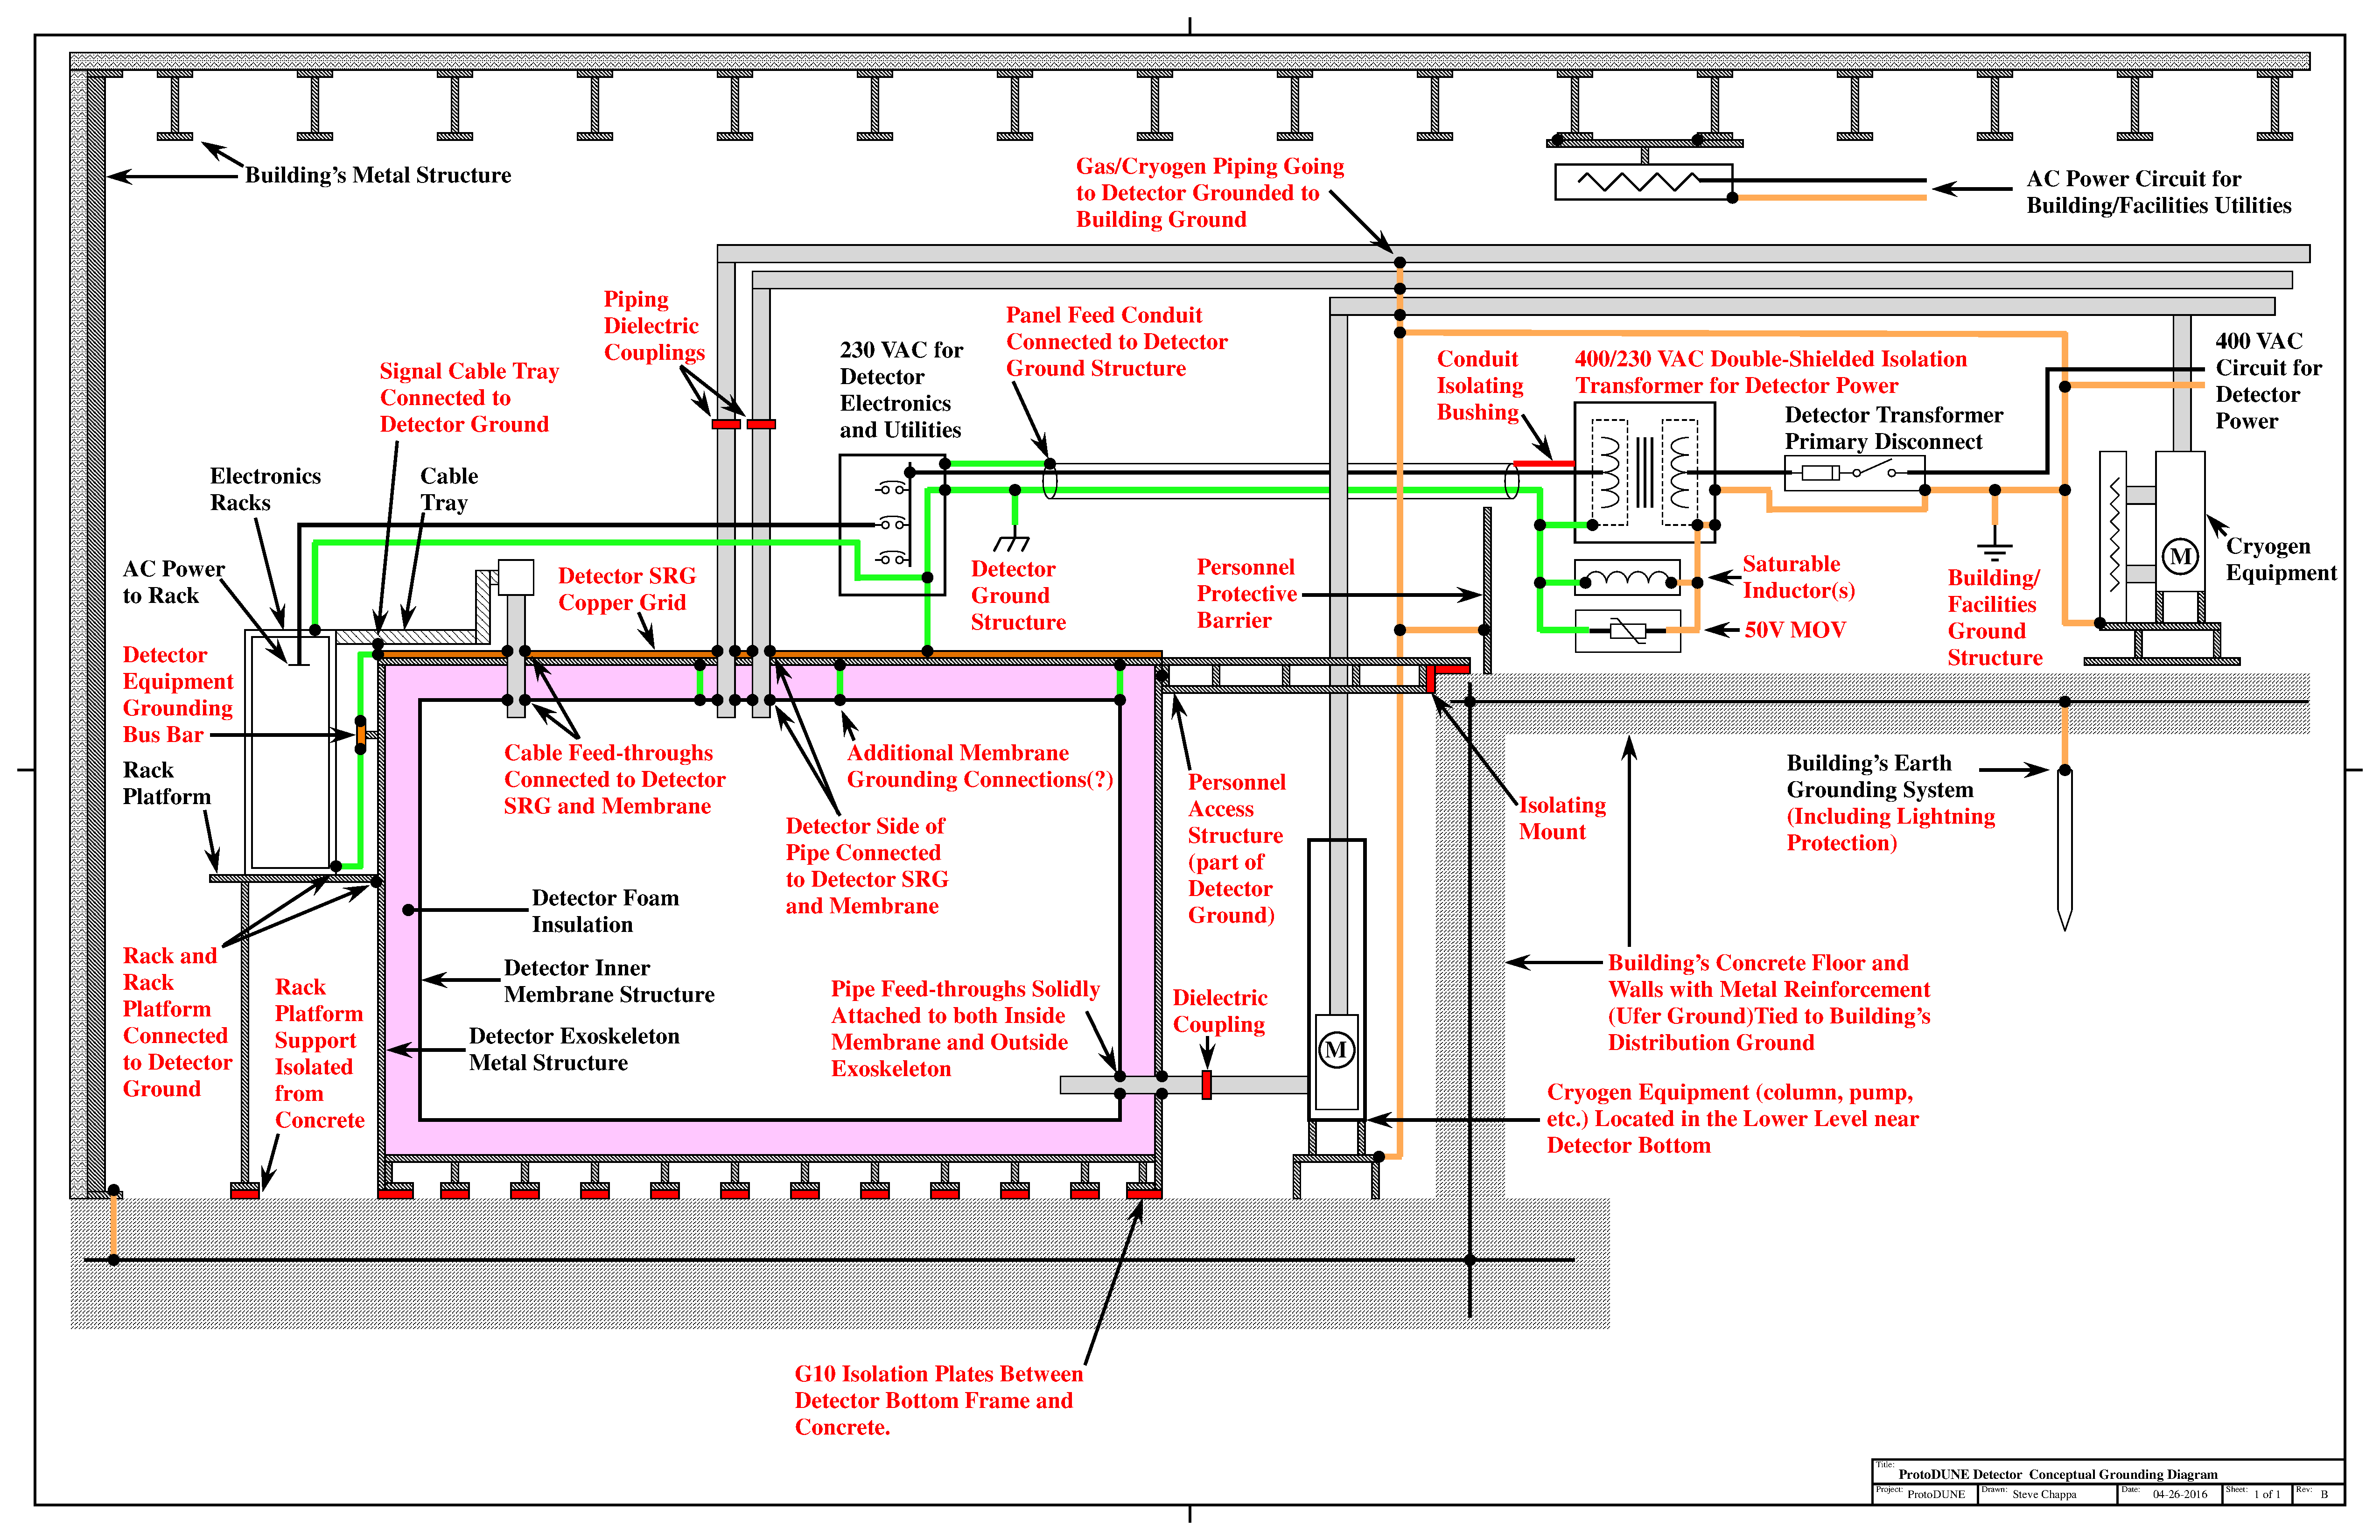
\includegraphics[angle=90, width=0.8\textwidth]{ProtoDUNE_GNDing_diagram_revB}
\end{cdrfigure}


\textbf{ProtoDUNE Grounding Points – Building and Detector Infrastructure}
\begin{itemize}
\item ProtoDUNE requires a ground structure which isolates the detector and local detector racks from all other electrical systems.
\item ProtoDUNE defines two distinct ground systems:  Detector Ground and Building Ground.
\item A safety ground, consisting of two or more saturable inductors, will connect the two ground systems and maintain a low impedance current path for equipment short circuit and ground fault currents.   This will insure personnel safety by limiting equipment/equipment and equipment/ground touch potentials.
\item Detector Ground consists of the steel containment vessel enclosing the cryostat, the cryostat, and all metal structures attached to or supported by the detector vessel. Dielectric breaks will be required on all cryo piping and any other metal structures which are referenced to Building Ground. 
\item Building Ground consists of the network of grounding bus bars and inter-connected rebar which exists in the ENH1 Facility.
\item An insulated barrier, ~0.10 inch G10, shall be installed between the floor of the facility and the bottom cryostat containment vessel to minimize low frequency ground and noise currents conducted between Building and Detector grounds.
\item Detector Readout racks should be located on top of/or near the top of the cryostat so that all the readout racks can be on a common Detector ground system and the cable runs minimized.
\item All cable trays going from the racks to the ports will be solidly connected to the top plate reference ground and will be considered part of Detector ground.
\item All cryo or gas piping, needs to be connected to Building ground at intervals before arriving at the cryostat. These pipes are required to have dielectric breaks located near the top of the cryostat.
\item A 230/400 VAC, double shielded, isolation transformer will be required, located close to the detector or on it. The service panel from this transformer will need surge protection.
\item All connections between the detector racks (Detector ground) and the Control room/barracks (Building ground) need to be optic fiber or isolated copper connections.
\item The top plate of the cryostat serves as the signal reference plane and Detector ground. A copper grid, solidly connected to all ports and to the racks, needs to be provided.
\item All local detector racks (not DAQ racks located in barracks) must be solidly connected to the platform and to the cryostat top reference grid/plane which represents Detector Ground.
\item Copper grounding bus bars should be provided near the racks and any other equipment mounted on the cryostat to aid in maintaining the low-impedance inter-connections to Detector ground.
\item All VFDs near the cryostat need careful design to prevent ground currents from coupling to the cryostat. 
\item The port penetrations need to utilize a “360-degree” connection to the outside surface of the cryostat and to the inside surface of the inner membrane.
\item The HV power supply needs to be mounted somewhere on or next to, the cryostat.
\item The HV cable shield needs to be solidly bonded to the cryostat. This shield must not be able to be charged up in the event of damage to the cable.
\end{itemize}

%%%%%%%%%%%%%%%%%%%%%%%%
\subsection{Power and rack space requirements}

ProtoDUNE power and rack space requirements are estimated for two areas.  The first area is for the equipment located on or near the detector and which is referenced to detector ground.  The second area is for the barracks computing room which will house the DAQ racks and an online disk buffer farm.

The detector rack requirements are estimated to be somewhere between 6 - 8 racks.  These racks will contain equipment for the high voltage drift power supply, APA wire bias power supplies, APA wire readout LV supplies, PD readout LV supplies, calibration systems, camera readout, scintillator counter readout and purity monitors.  A rough power estimate for this area is ~50KVA, and the plan is to order a 75KVA isolated double shielded transformer to supply all detector power needs.  All detector racks will be air cooled.

The DAQ Computing Room is located in a barracks building as shown in figure \fixme{7}.  The power to this room should be supplied by building infrastructure.  It is estimated that a total of 6 racks will be required with a total power estimate of about 12KVA.  The computers in this room will require air conditioned racks.
%
\begin{cdrfigure}[short caption for table of figures]{label}{8 long caption that appears below picture}
%  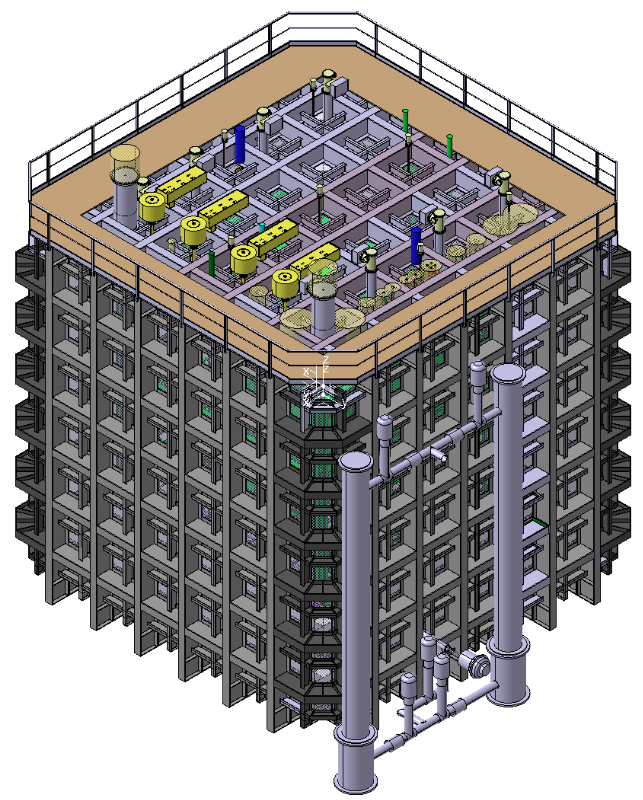
\includegraphics[width=0.8\textwidth]{protoDUNE_cryostat.png}
\end{cdrfigure}
%


%%%%%%%%%%%%%%%%%%%%%%%%%%%%%%%%%%%%%%%%%%%%%%
\section{Cooling requirements}
cooling water \\
chilled air\\



space and infrastructutre requirements in the EHN1 area

